
\chapter{Introduzione}

\section{Motivazione}
% Spiegare il perché l'ho fatto Dati importanti, piccole e medie imprese devono sfruttare software opensource disponibili a tutti che permetto di passare da una frase experimental a production ready

Le piccole e medie imprese sono sempre più informatizzate e dipendenti da servizi informatici per poter svolgere il loro lavoro. Per questo motivo scoprire e analizzare il traffico anomalo in transito sulle reti aziendali è sempre più importante, il nostro obiettivo è farlo ad un basso costo, senza aggiungere hardware o applicativi che richiedano molta potenza di calcolo o di banda, sfruttando i router che compongono la rete. Punteremo a scoprire le anomalie nei dati di rete sui singoli flussi e nei dati aggregati analizzando alcune metriche su un server aggiuntivo che si occuperà anche di mitigare l'attacco informando i router sui flussi da bloccare o limitare.
Gli attacchi maggiormente presi in considerazione in questa tesi saranno gli attacchi di ``Distributed Denial of Service'', ma gli stessi principi potranno essere applicati anche ad altre tipologie di anomalie.
% problema delle botnets
Inoltre l'analisi dei dati raccolti sull'utilizzo della rete potrà portare anche alla risoluzioni di problemi di rete non derivanti da attacchi.

\section{Collaborazione con Tiesse s.p.a.}

Questa tesi è stata sviluppata in collaborazione con Tiesse s.p.a.: un'azienda che progetta e realizza, interamente in Italia, router e dispositivi M2M, con connettività wired e mobile.

L'azienda ha oltre 20 anni di esperienza, ed è stata riconosciuta come uno dei maggiori fornitori di CPE a banda larga e wireless su reti 3G/4G dalla maggior parte delle compagnie telefoniche. Oltre alla produzione e alla progettazione di router e apparecchiature di rete, sviluppa progetti custom, sia hardware che software. I prodotti Tiesse sono particolarmente adatti ad applicazioni Business e Mission Critical per il Corporate Networking.

L'azienda è sempre attiva sull'aspetto di ricerca e sviluppo, anche tramite collaborazioni con il Politecnico di Torino e in particolare negli ultimi anni ha messo il focus su soluzioni software per la sicurezza e l'analisi dei dati di rete.

La sede centrale dell'azienda si trova ad Ivrea, ma possiede anche sedi distaccate a Torino, Avezzano e Roma.

% Scrivo quello dell'abstractafd
% lavoro svolto in collaborazione e in parte in presenza presso l'azienda spa di Ivrea

% Sezione in cui parlo di cui fa Tiesse spa
% - presento azienda
% - location e sedi distaccate
% - parlare della collaborazione con il poli => sempre in collaborazione per ricerca e sviluppo in particolare negli ultimi anni con un focus sugli aspetti di sicurezza e analisi dati di rete e non solo hw => prendere spunto anche dal sito
% - prendere ispirazione dalla slide tiesse di itasec

\section{Scenario}
\begin{figure}[]
    \label{fig:scenario}
    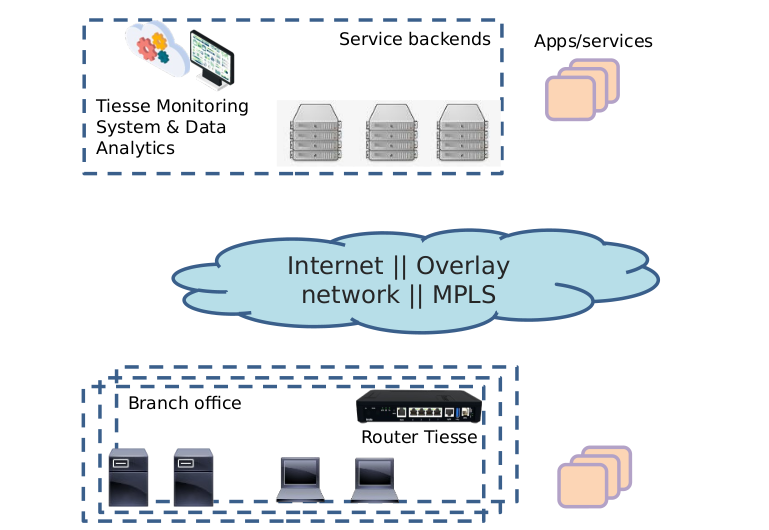
\includegraphics[width=\hsize]{images/introduzione/scenario_2.png}
    \caption{Scenario rete Tiesse e clienti}
    \centering
\end{figure}

Nello sviluppo della nostra soluzione abbiamo preso in considerazione un tipico scenario aziendale, in cui esiste una sede centrale, ben protetta e su cui sono ospitati i servizi dell'azienda e tante sedi periferiche: uffici, negozi o altro, collegati ai servizi della sede centrale tramite un overlay MPLS o una VPN.
Le sedi periferiche sono quelle più esposte sotto l'aspetto della sicurezza, \uline{anche solo per il fatto che sono in numero maggiore, spesso non ci sono i responsabili dell'IT in sede e solitamente sono meno controllate rispetto la sede centrale}. Per questo motivo il nostro obiettivo è quello di proteggere i servizi, gli applicativi aziendali e la rete centrale dai dispositivi malevoli connessi alle reti degli uffici.
L'organizzazione di Tiesse e di molti suoi clienti è caratterizzata dallo scenario in figura \ref{fig:scenario}. Utilizzando questa struttura di rete per effettuare la raccolta, l'analisi del traffico e le prove, ci siamo basati su un esempio di sede periferica, nel nostro caso un ufficio dell'azienda situato a Torino, con l'obiettivo di proteggere i servizi aziendali presenti nella sede centrale di Ivrea a cui l'ufficio è collegato tramite una VPN.

Un altro caso possibile di utilizzo di questa soluzione è la distribuzione dei servizi in cloud, in cui l'azienda non ha il controllo dell'infrastruttura di rete e sfrutta i router thrusted nelle reti degli uffici per analizzare il traffico.


\begin{figure}[]
    \label{fig:scenario_2}
    %https://lucid.app/lucidchart/8119c7e9-e2e1-4dbb-b55f-bebf6c97af2d/edit?beaconFlowId=3612F8C43004D8D2&page=0_0#
    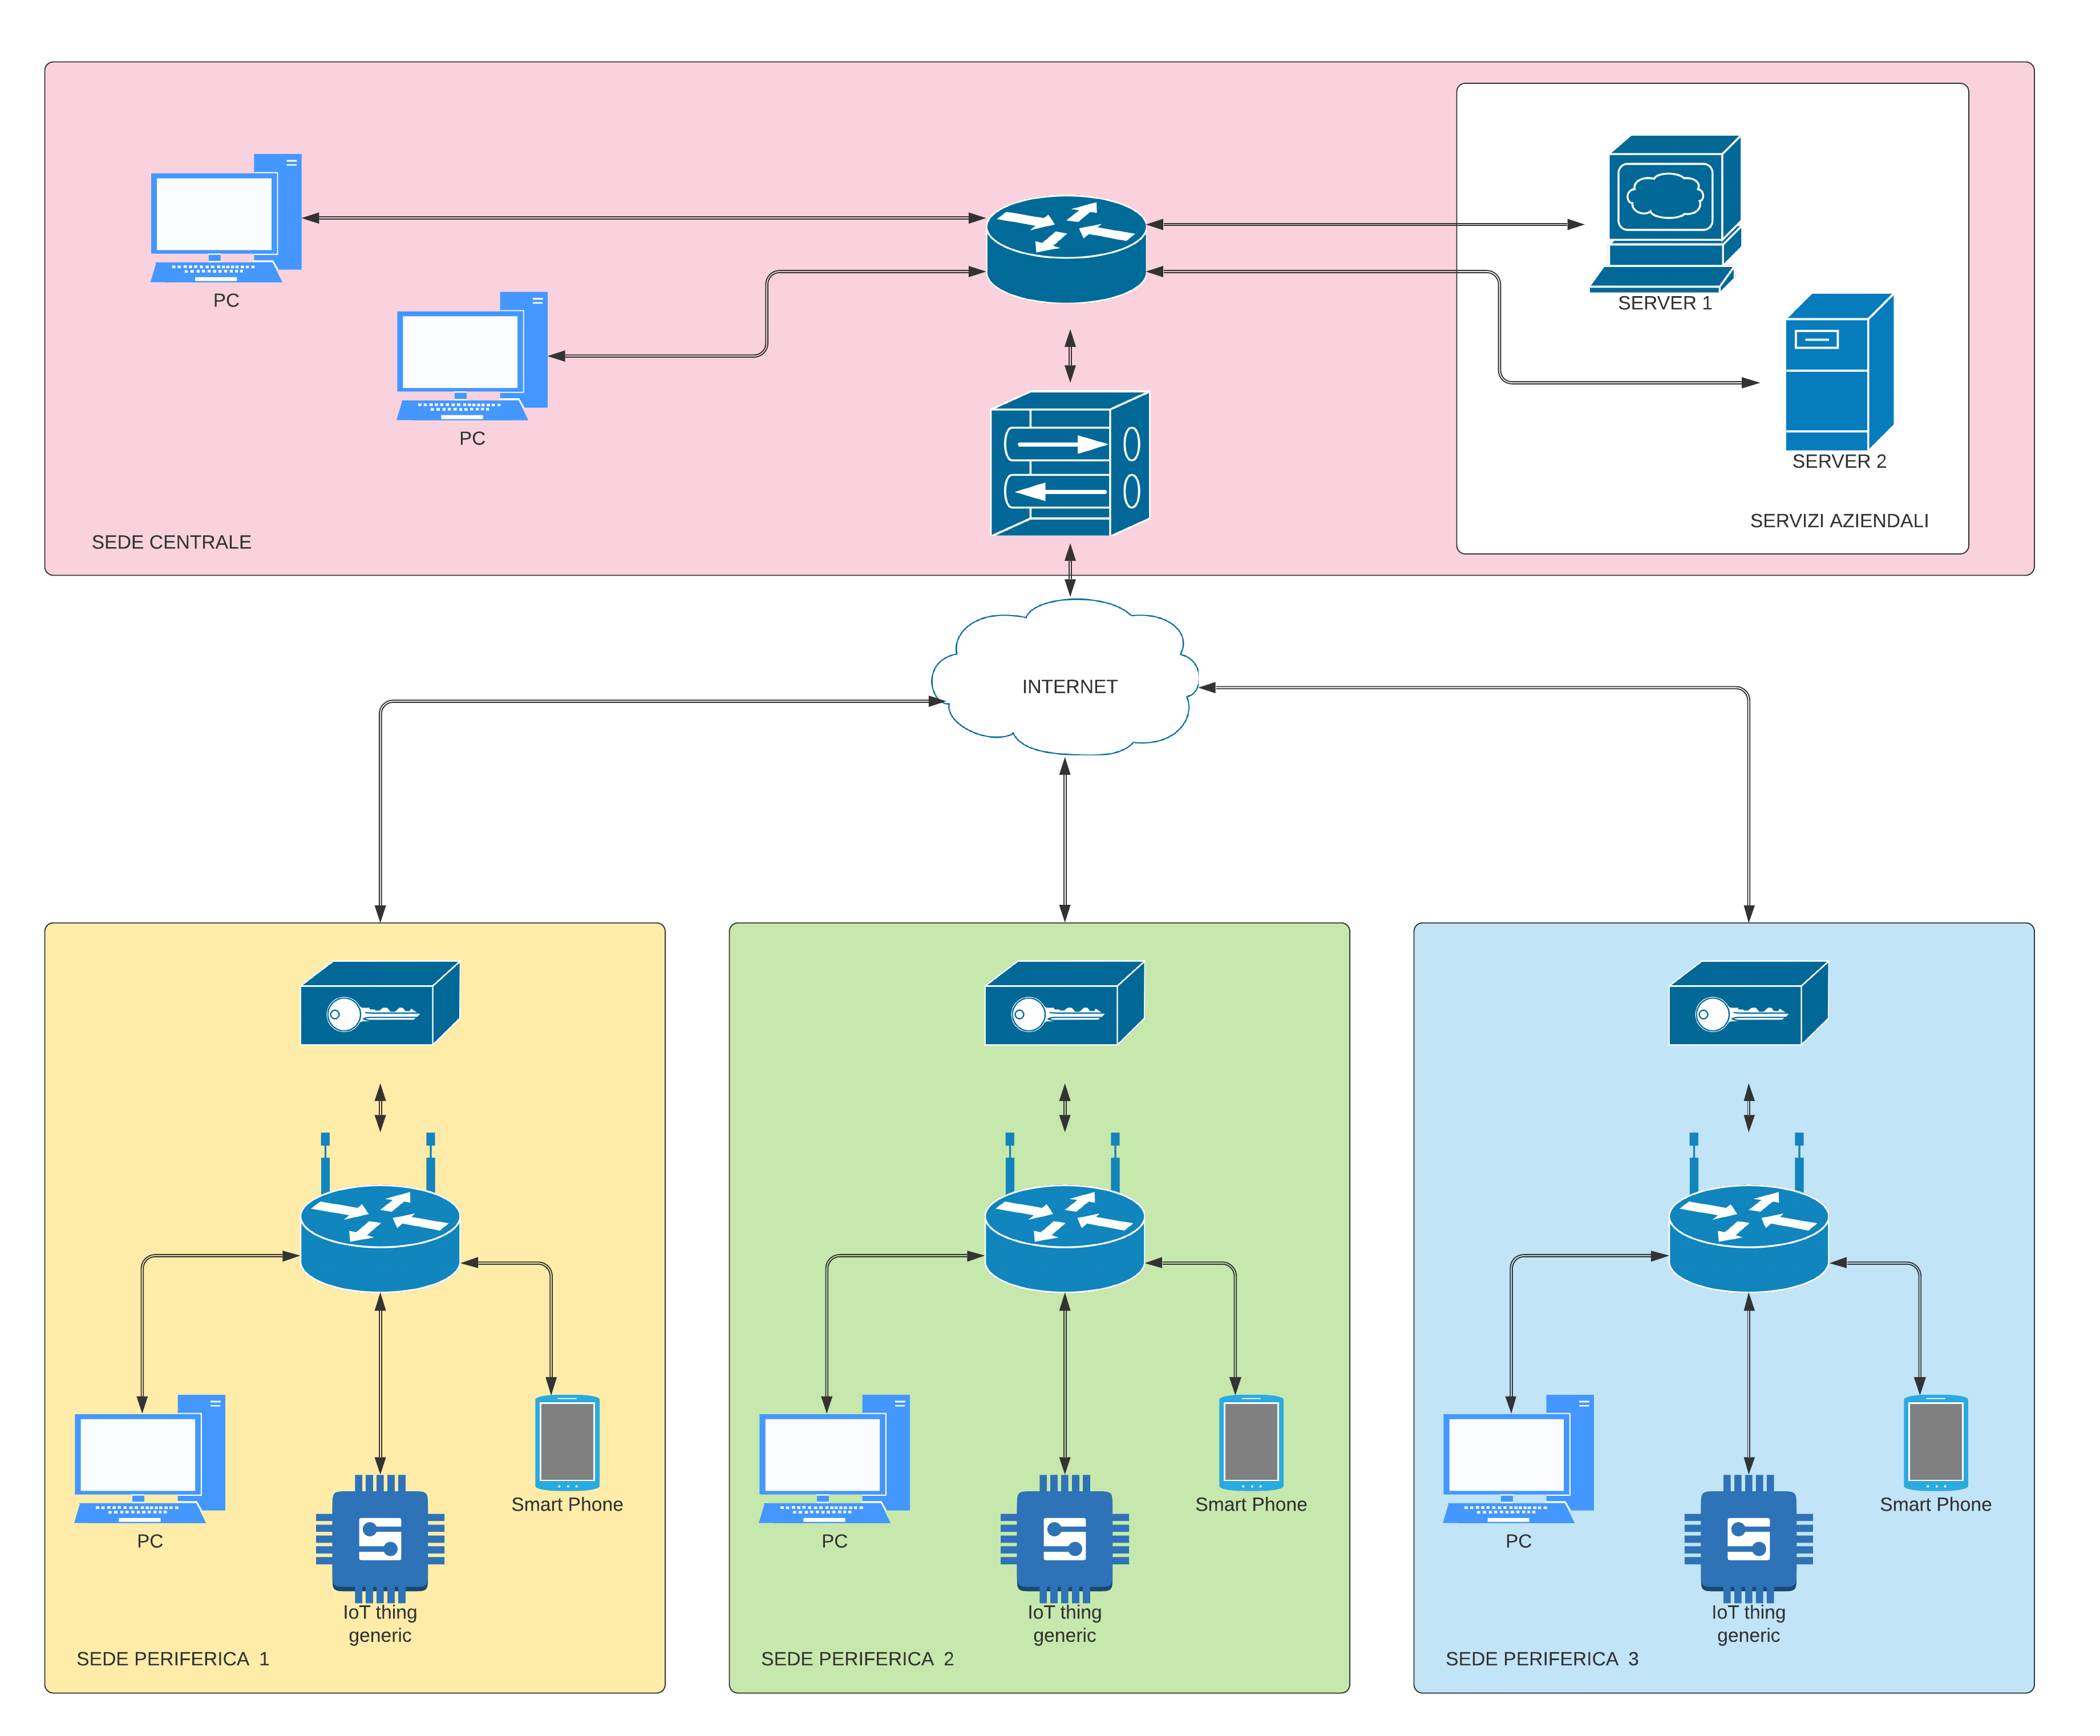
\includegraphics[width=\hsize]{images/introduzione/scenario.png}
    \caption{Scenario rete Tiesse e clienti}
    \centering
\end{figure}


\section{Gli attacchi DDoS}

Gli attacchi di Denial of Service (DoS) sono attacchi nel campo della sicurezza informatica che mirano a interrompere la fruizione di un servizio, fornito da un host connesso a internet, da parte di utenti legittimi. L'attacco ha l'obiettivo di esaurire le risorse dell'host in modo da non consentirgli di erogare le risposte ai richiedenti.
Nel caso in cui la sorgente del traffico che genera traffico malevolo per creare disservizi non sia unica, si parla di attacchi di denial of service distribuiti (Distributed Denial of Service).

\subsection{Tipologia di attacchi DDoS}
    
Gli attacchi DDoS possono essere suddivisi in due categorie principali in base al loro funzionamento. La prima si basa sul mandare alla vittima pacchetti malformati in grado di sfruttare un bug o una falla a livello applicativo. La seconda categoria invece si basa su tecniche utili a colpire l'infrastruttura del servizio, per il funzionamento di questa tecnica vengono usati uno o entrambi i seguenti metodi: il primo si basa sull'interruzione della connessione di rete grazie all'esaurimento della banda o della capacità di processamento dei router o di entrambe, nel secondo caso l'obiettivo dell'attaccante è di esaurire le risorse (es. sockets, CPU, memoria) del server che ospita il servizio \cite{ddos_survey_1}.

\begin{figure}[h]

    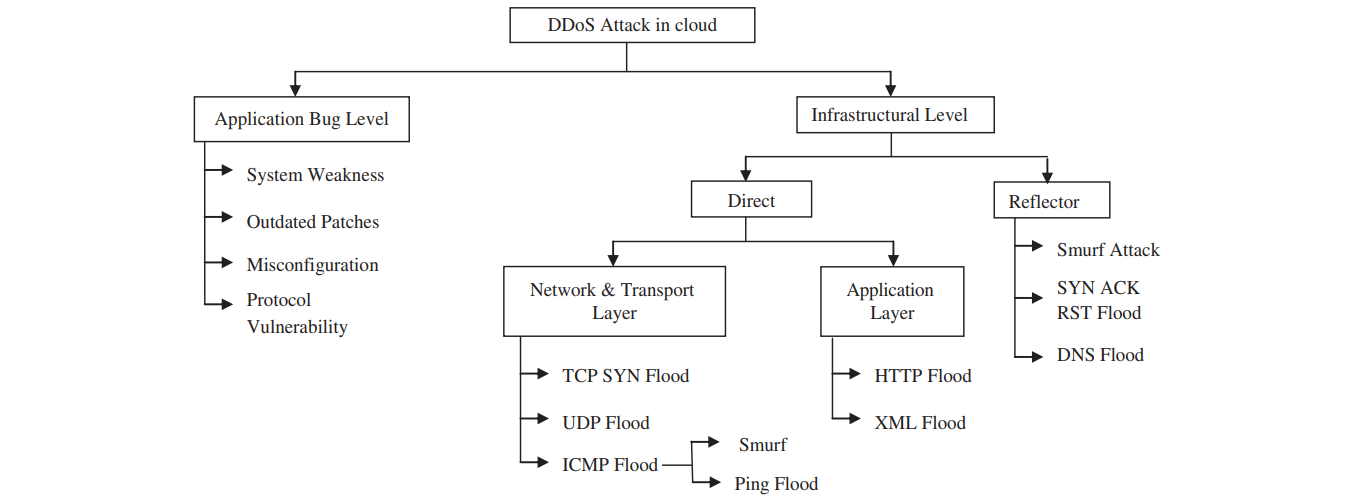
\includegraphics[width=\hsize]{images/introduzione/tipologie_ddos.png}
    \caption{Tipologie di attacchi DDoS \cite{ddos_survey_3}}
    \centering
\end{figure}

L'obiettivo di questa tesi sarà concentrato sul rilevamento e la mitigazione della seconda categoria di attacchi, basata sull'esaurimento delle risorse.

\subsubsection{Attacchi basati sul flooding}

\begin{figure}[h]
    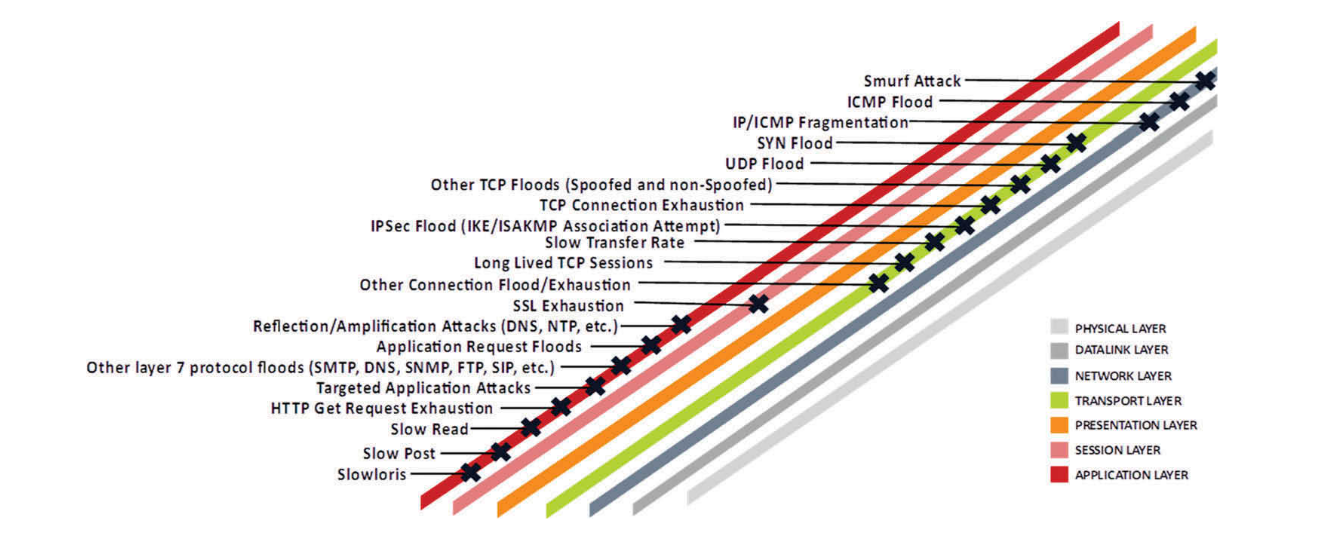
\includegraphics[width=\hsize]{images/introduzione/attacchi_per_livello.png}
    \caption{Attacchi per livello \cite{ddos_survey_4}}
    \centering
\end{figure}

\paragraph{Network/transport-level DDoS flooding attacks} % todo: rivedere titolo
Gli attacchi di denial of service che mirano ad esaurire le risorse di rete si basano sull'invio di molti pacchetti con lo scopo di consumare totalmente \uline{la banda o le socket} della vittima, queste tipologia di attacco può essere effettuata in maniera diretta: \emph{flooding attacks} e \emph{protocol exploitation attacks}, nel primo caso la vittima viene inondata di pacchetti (UDP flood, ICMP flood, DNS flood, VoIP flood an etc.), in questo caso la banda aggregata in uscita di tutti gli attaccanti deve essere superiore a quella del servizio che si vuole danneggiare, nel secondo caso vengono sfruttane delle caratteristiche dei protocolli della vittima in modo da consumare una grande quantità di risorse (es. TCP SYN flood, TCP SYN-ACK flood, RST/FIN flood e ecc).

Gli attacchi che non vengono effettuati in maniera diretta invece sfruttano la riflessione o l'amplificazione: nei \emph{Reflection-based flooding attacks} chi attacca manda un particolare pacchetto, indirizzandolo ad un riflettore e questo riflettore manda le sue risposte alla vittima, in modo da esaurirne le risorse. Un esempio di questa tipologia di attacchi sono lo Smurf e il Fraggle, nel primo vengono mandati ICMP Echo Request ad una sottorete, usando come ip di destinazione l'indirizzo broadcast e specificando come ip sorgente l'ip della vittima, utilizzando l'ip spoofing, causando la risposta di tutti gli host verso l'indirizzo della vittima \cite{ddos_survey_2}.
Gli \emph{Amplification-based flooding attacks} sfruttano servizi che restituiscono risposte più grandi della richiesta ricevuta, un esempio è il DNS amplification, che riesce a moltiplicare dalle 30 alle 50 volte\cite{imperva_amplification} la banda in uscita dell'attaccante, il suo funzionamento si basa sull'utilizzo dell'ip spoofing mandando un pacchetto con indirizzo ip sorgente della vittima, così il servizio DNS risponderà ad essa con un flood di pacchetti di dimensioni maggiori \cite{ddos_survey_1}. Lo stesso principio è sfruttato anche dal NTP amplification che può aumentare il traffico con un rapporto tra 20:1 e 200:1, arrivando in alcuni casi anche a 556:1 \cite{imperva_amplification}. 

% todo: Amplification-based flooding attack, negli attacchi di rete: qua non so giustificarla bene pagina 3 \cite{ddos_survey_1}
% qua parla bene del fattore di moltiplicazione degli attacchi https://www.imperva.com/blog/ntp-flood-explained/

\paragraph{Application-level DDoS flooding attacks} % todo: rivedere titolo
% qua taglio un po' corto sugli attacchi applicativi perché approfondirò maggiormente quelli di rete
Gli attacchi DDoS al livello applicativo hanno lo scopo di terminare le risorse del server(cpu, memory, disk/db bandwidth, I/O bandwidth),  solitamente usano meno banda rispetto gli attacchi rivolti verso l'infrastruttura di rete rete, per questo motivo è anche più difficile identificarli. Le tecniche utilizzate sono simili alle precedenti. Degli esempi sono l'HTTP flooding che effettuando l'invio di molte richieste HTTP, obbliga il server a produrre risposte che possono essere computazionalmente pesanti, oppure possono sfruttare l'SQL Injection per imporre un lock sul database e bloccare il funzionamento dell'applicazione. Altri attacchi di questa tipologia possono essere l'HTTP fragmentation, lo slowpost attack, slowreading attack e lo slowloris attack, tutte tecniche che mirano a mantenere molte connessioni aperte mandando o ricevendo pochi dati per volta \cite{ddos_survey_1}.
Gli attacchi di tipo applicativo sono molto eterogenei e non possono essere mitigati a livello di rete/trasporto, per questo motivo questa tesi prenderà in considerazione solo gli attacchi trattati al paragrafo precedente.

\paragraph{DDoS con obiettivo la riduzione della qualità del servizio}
\label{paragraph:ddos_degradation}
% parlare anche di attacchi a basso rate, ma da molte fonti che portano ad un grande risultato finale \cite{ddos_survey_4,ddos_survey_3} pagina 38, rendendolo difficile da indentificare

L'unico obiettivo possibile degli attacchi DDoS non è la sola interruzione del servizio, ma un altro risultato attuabile è la degradazione del servizio, consumando una parte di risorse destinate agli utenti legittimi e creando loro ritardi nelle risposte. Questo risultato può essere raggiunto utilizzando dei packet rate più bassi, e di conseguenza meno rilevabili o dei l'invio d flood di pacchetti con rate variabili \cite{ddos_survey_3, ddos_survey_4}.
Gli approcci a bassi rate sono utilizzati frequentemente dagli attacchi DDoS a larga scala, poichè l'aggregazione di moltissime fonti a basso rate portano comunque ad un grande risultato finale.

\subsection{Vittime attacchi DDoS}

% todo: introduzione: qua potrei nominare delle statistiche sugli attacchi con la distribuzione delle vittime
\begin{figure}[h]
    % todo: capire come gestire citazioni immagini a livello di copyright
    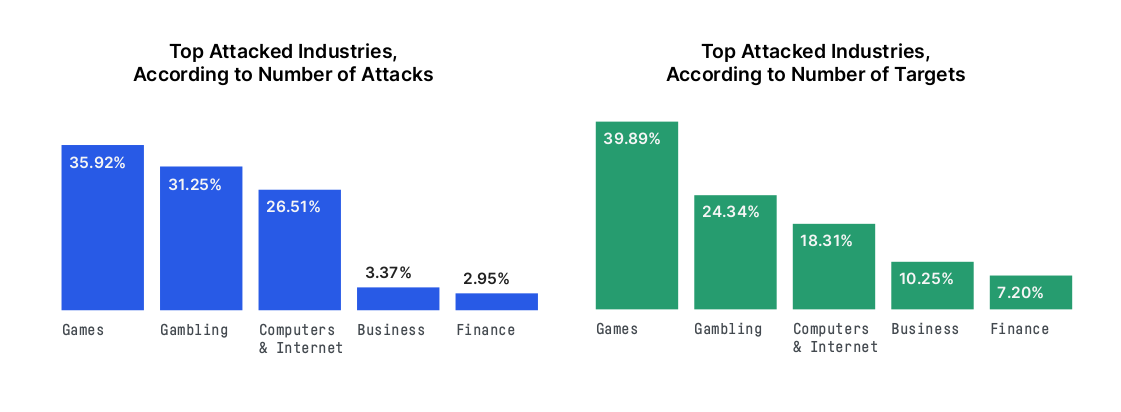
\includegraphics[width=\hsize]{images/introduzione/bersagli_ddos.png}
    \caption{Distribuzione vittime DDoS, 2020 \cite{imperva_ddos_report}}.
    \centering
\end{figure}

I target degli attacchi DDoS possono differenziarsi molto: da un utente domestico ad un governo \cite{ddos_motivations}. Per capire maggiormente chi possono essere le vittime di un attacco bisogna analizzare le motivazioni che spingono gli attaccanti e con le diverse motivazioni si può anche capire qual'è il rischio per quanto riguarda la portata dell'attacco. 

Per semplicità possiamo suddividere gli incentivi di un attacco in cinque principali categorie \cite{ddos_survey_1, ddos_motivations}:

\begin{itemize}
    \item Beneficio economico o finanziario: sono gli attacchi riguardanti principalmente le aziende, sono considerati i più pericolosi e difficili da fermare. Mirano ad ottenere benefici finanziari dagli attacchi e i creatori dell'attacco sono abitualmente persone con esperienza.
    \item Vendetta: questa tipologia di attacchi sono mesi in atto da persone, solitamente con uno scarso livello tecnico, a fronte di un'apparente ingiustizia percepita.
    \item Credo ideologico: alcuni attaccanti si trovano ad effettuare attacchi contro alcuni obiettivi per motivi ideologici. È una motivazione di attacco meno comune delle altre, ma può portare ad attacchi di grande entità. % todo: valutare se mettere esempi attacchi tipo cnn 2008, wikileaks 2010 e iran 2009
    \item Sfida intellettuale: gli utenti che sviluppano attacchi per questa motivazione vogliono imparare e sperimentare a lanciarli. Spesso sono giovani appassionati di hacking che grazie alla facilità con cui si possono affittare botnets o utilizzare semplici tool riescono ad effettuare con successo DDoS.
    \item Cyberwarfare: gli attaccanti di questa categoria appartengono ad organizzazioni terroristiche o militari di un paese e sono politicamente motivati ad attaccare risorse critiche di un altro paese. Un grande numero di risorse viene usato per questa tipologia di attacco e può paralizzare le infrastrutture critiche di un paese, portando ad un grave impatto economico.
\end{itemize}


Le maggiori vittime secondo il report \cite{imperva_ddos_report} sono le compagnie che operano del campo dei videogiochi e delle scommesse, entrambe comportano un grande livello di rischio e spesso i giocatori si rifiutano di seguire le regole. Le aziende che incentrano il loro business sul settore di Internet e della computazione si trovano al terzo posto, seguiti dalle attività commerciali e da quelle finanziarie.


\subsection{Diffusione attacchi DDoS}


\begin{figure}[h]
    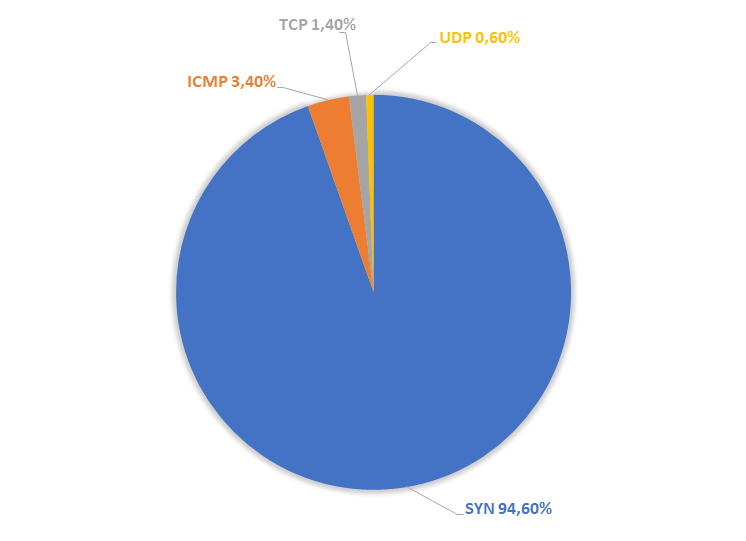
\includegraphics[width=\hsize]{images/introduzione/tesi_distribuzione_tipologia_attacchi.png}
    \caption{Distribuzione di attacchi DDoS per tipologia, Q3 2020 \cite{ddos_kaspersky_q3_2020}}
    \centering
\end{figure}

Nel mondo a fine 2020 la quasi totalità degli attacchi DDoS proviene da botnets, con target principali in Cina e negli Stati Uniti. Le tipologie di attacco maggiormente utilizzate sono il \emph{Syn Flood} che copre più del 90\% della totalità degli attacchi, seguito da \emph{ICMP flooding} e \emph{UDP flooding} \cite{ddos_kaspersky, ddos_kaspersky_q3_2020}.


La maggior parte degli attacchi DDoS hanno una portata inferiore ai 10 Gbps (circa il 65\%), ma il 3\% di essessi raggiunge cifre incredibili, superiori al 200 Mbps \cite{imperva_ddos_report}.

\begin{figure}[h]
    % todo: capire come gestire citazioni immagini a livello di copyright
    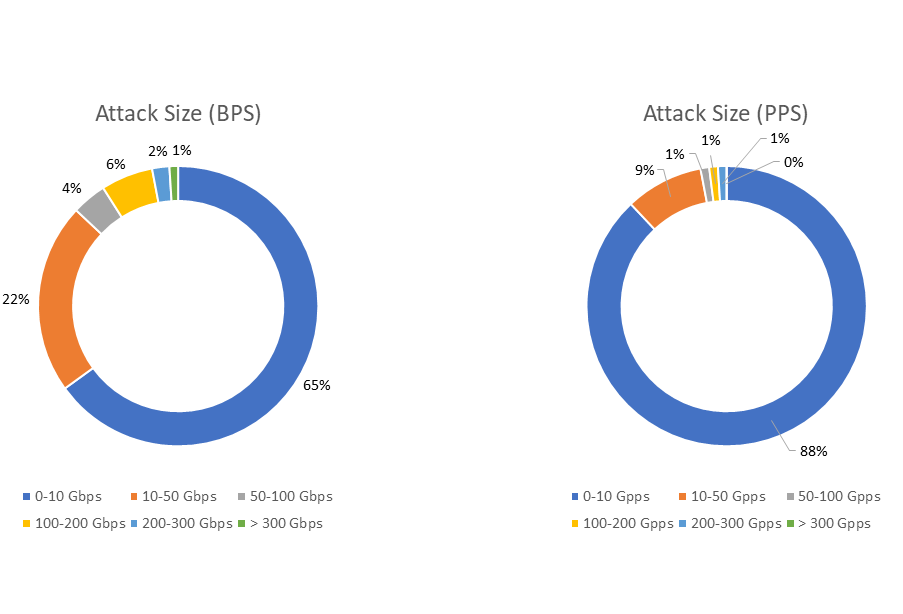
\includegraphics[width=\hsize]{images/introduzione/attacks_size_2.png}
    \caption{Distribuzione di attacchi DDoS per dimensione, 2020 \cite{imperva_ddos_report}}
    \centering
\end{figure}


\subsubsection{Attacchi basati su botnets}

Gli attacchi basati su botnets sono un grande problema per l'implementazione di sistemi anti-DDoS perché un grande numero di ``zombie'' rende l'attacco più distruttivo, in aggiunta spesso utilizzano ip spoofing complicando il tracciamento all'indietro per determinare la vera locazione bot \cite{ddos_survey_1}.

Il funzionamento delle botnet si basa su tre fasi. La prima consiste nel reclutamento ``dell'esercito'': fase in cui vengono contagiati i dispositivi tramite worms (programmi che si autopropagano) che sfruttano falle nella sicurezza. Sono usate tecniche come: la scansione automatica di indirizzi ip casuali per trovare altri soggetti vulnerabili, questa tipologia di scansione però produce molto traffico e può rendere possibile rilevare l'attacco, oppure una hitlist: una tecnica che frutta una lista di possibili macchine potenzialmente vulnerabili, la scansione della subnet o l'utilizzo di informazioni dei target basandosi sulle informazioni contenute nelle vittime infettate dai wormc.


% qui dovrei magari differenziare le botnet controllate direttamente e indirettamente e dilungarmi meno, magari nominare le tre fasi degli attacchi  \cite{ddos_motivations} pagina 5 \cite{ddos_survey_4} pagina 37
Nella fase successiva alla creazione di un ``esercito'' avviene la propagazione delle informazioni riguardanti le vittime da attaccare, con la durata e l'ora.
I bot possono essere controllati dell'artefice dell'attacco tramite tre architetture \cite{ddos_survey_4}: % pagina 46
\begin{itemize}
    \item IRC-based: architettura client-server in cui ad ogni server si possono collegare centinaia di dispositivi, utilizza un protocollo testuale e utilizzando porte non standard rendendo molto difficile il riconoscimento del comando per lanciare un DDoS, il quale si può nascondere facilmente nel grande traffico dei server IRC. Il singolo server a cui si connettono tutti i client può essere considerato un single point of failure.
    \item Web based: ogni bot scarica periodicamente delle informazioni tramite una richiesta web ad un server, i comandi di questa tipologia di controllo sono i più difficili da tracciare.
    \item P2P based: le moderne botnet utilizzano una struttura più robusta e flessibile, invece di avere un singolo server centrale al controllo della botnet, viene mandato un comando in broadcast a tutti gli agent. Questo le rende più affidabili, poiché l'eliminazione di un agent non rende la rete non funzionante, ma al tempo stesso rende il mantenimento della rete più difficile e la scoperta di un agent può rivelare tutti gli altri. 
\end{itemize}
L'ultima fase è il tentativo di attacco vero e proprio.

\begin{figure}[h]
    % todo: capire come gestire citazioni immagini a livello di copyright
    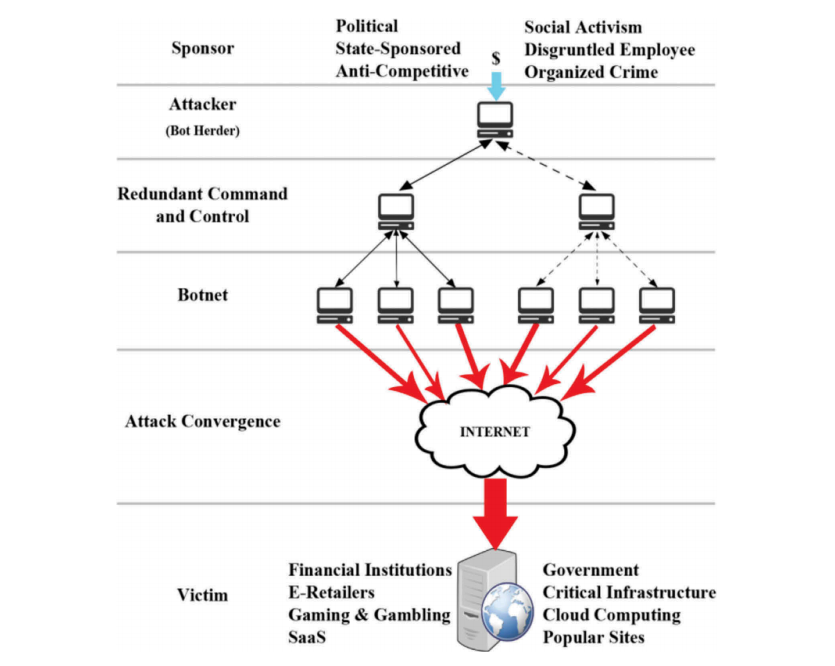
\includegraphics[width=\hsize]{images/introduzione/struttura_botnets_2.png}
    \caption{Struttura di lancio di attacchi DDoS \cite{ddos_survey_4}.}
    \centering
\end{figure}

Un esempio di botnet è Mirai, una rete di dispositivi creata attraverso un malware che sfrutta le vulnerabilità dei dispositivi IoT per creare host malevoli da utilizzare in attacchi DDoS di larga scala. Il codice sorgente del bot è stato rilasciato pubblicamente nel 2016, questo ha permesso la creazione di molte sue varianti, lasciando a chiunque la possibilità  di crearsi la propria botnet.
Il codice per effettuare attacchi DDoS include dieci tipologie diverse di attacco, ognuna configurabile in molti modi e lanciabile attraverso l'utilizzo di un server di comando e controllo \cite{slide_mirai}.

Alcuni attacchi possibili tramite la botnet Mirai sono: flood DNS, STOMP: una attacco che mira ad effettuare il three-way TCP handshake e solo dopo quando la sessione sarà messa in whitelist inizia un ACK flood, GREIP: incapsula nel pacchetto GRE un pacchetto ip con ip sorgente e destinazioni casuali, SYN flood, ACK flood, UDP flood e HTTP flood.

\subsubsection{Attacchi DDoS famosi}

%todo: qua parla del flood dns https://www.cloudflare.com/it-it/learning/ddos/dns-flood-ddos-attack/

Aggiungo questa parte o sarebbe superflua?

Potrei parlare dei primi attacchi, fino a quelli moderni menzionando i motivi dell'attacco se scoperti, la tipologia e la portata.


\section{Organizzazione della tesi}

La tesi nei successivi capitoli tratterà lo stato dell'arte dei sistemi anti-ddos esistenti (capitolo 2), mostrando come è possibile riconoscere un attacco e dove è meglio farlo per poterlo mitigare al meglio. Nel capitolo 3 approfondirà maggiormente lo stato dell'arte dei sistemi di anomaly detection da utilizzare per rilevare un attacco DDoS.
Nei capitoli 4 e 5 verrà illustrata la soluzione da noi proposta, focalizzandosi nel quarto sulla tecnica per rilevare un'anomalia e nel quinto su come mitigarla.
Nel capitolo 6 vengono menzionati possibili lavori futuri e nel 7 le conclusioni con delle considerazioni sulla soluzione proposta.